\chapter{Simulations}

Simuler des images réalistes est un enjeu important en imagerie médicale. Le fait d'avoir accès à la vérité terrain, contrairement à la routine clinique, permet de valider des hypothèses de manière beaucoup plus fine. De plus, avec l'augmentation des performances de ordinateurs et l'accès à des centres de calculs, il devient possible de créer des bases de données de patients de plus en plus importantes et réalistes.

Nous allons tout d'abord présenter les différents types d'algorithme de simulations disponibles. Ensuite, nous feront un état de l'art des simulateurs développés par la communauté. Enfin, nous décrirons le simulateur retenu ainsi que les contributions réalisées pour générer la base de données.

	\section{principe des simulations}

		\subsection{Simulations analytiques}

Les simulateurs analytiques utilisent des approximations fortes pour résoudre les problèmes de manière analytique. Il ne simulent pas de manière réaliste le déplacement des particules (positon, photon) comme les simulateurs Monte-Carlo.

Dans le cas de l'imagerie TEP, la simulation analytique revient à réaliser des projections du volume TEP dans l'espace du sinogramme. Ce sinogramme est ensuite bruité et modifié pour prendre en compte les effets des coïncidences aléatoires et des photons diffusés. L'efficacité des détecteurs est aussi prise en compte, tout comme les effets de l'atténuation. 

La reconstruction est ensuite réalisée de manière classique à l'aide des algorithmes de reconstruction TEP.


Cependant, bien que ce type de simulateur soit extrêmement rapide, les images générées ne parviennent pas à reproduire de manière parfaite les différents phénomènes physiques à l'origine du bruit.




		\subsection{Simulation Monte Carlo}

Les simulations Monte-Carlo~\footnote{Le nom de Monte-Carlo fait allusion aux jeux de hasards pratiqués dans la ville du même nom} (MC) ont une approche probabiliste en modélisant la trajectoire de chaque photon indépendamment. .

Dans le cadre de l'imagerie TEP, le modèle probabiliste est appliqué à l'émission, puis au parcours du positon, à son annihilation, ainsi que les interactions et la probabilité de détection des photons dans les détecteurs.

La génération et le suivi de chaque photon ainsi que de chaque désintégration prennent un temps extrêmement important, amplifié par le fait que deux désintégrations successives dans des organes différents peuvent amener à une coïncidence fortuite. Il faut aussi prendre en compte les limitations de l'électronique (incapacité à séparer des évènements trop proches en temps comme en énergie, saturation des capteurs, \dots)ce qui amène à des temps de simulation prohibitifs de l'ordre de plusieurs mois, même sur des centres de calculs. Le grand Challenge TERA 10 crée en 2006 a mobilisé un supercalculateur comprenant 7000 processeurs pendant 3h pour simuler une image corps entier à l'aide du simulateur GATE, avant la mise en place des procédures d'accélérations. Cela revient à plus 10 jours de calculs ininterrompus pour une soumission sur centre de calculs avec 100 processeurs disponibles en permanence.

	\subsection{Simulation Monte Carlo accélérées}

Les simulateurs Monte-Carlo accélérés utilisent des heuristiques pour augmenter la vitesse des calculs, notamment en réalisant des calculs préliminaires afin de simplifier les simulations futures. 

La séparation des simulations entre les coïncidences directes et diffusées, à l’aide des statistiques créées précédemment, permet encore d’accélérer les calculs. Le projet ANR fGATE a permis une amélioration des temps de calculs d'un facteur 20 par rapport à ceux présentés ci-dessus.

	\section{\'Etat de l'art des simulateurs TEP}

De nombreux simulateurs ont été développés par la communauté. Ils sont souvent développés à partir d'une librairie dédiée aux calculs de trajectoires de particules, comme GATE~\cite{jan2004gate}, qui se base sur le jeu d'outils de simulation d'interactions particule/matière Geant4~\cite{allison2006geant4}, le simulateur Penelo-PET\cite{espana2009penelopet} basé sur la librairie de simulation  PENELOPE~\cite{salvat2006penelope}, ou encore EGS-PET. L’université de Washington développe le simulateur Monte Carlo simSET ainsi que le simulateur analytique ASIM. 

De très nombreux simulateurs ont été développés en interne par de petites équipes pour les besoins des laboratoires, mais ils s'oriente actuellement  vers GATE, qui bénéficie d'un développement rapide et d'une grande communauté.

Une étude décrit l'ensemble des codes disponibles en 2002~\cite{buvat2002monte}, et a été mise à jour en 2006~\cite{buvat2002monte} pour prendre en compte les avancées techniques réalisées.

Nous avons utilisé PET-SORTEO, car il a été développé pour augmenter la vitesse de simulations et profiter de la parallélisation offerte par les centres de calculs. De plus, nous avons réalisé à CREATIS la première version de la base de données OncoPET\_BD~\cite{tomei2010oncopet_db} sur ce simulateur, ce qui permet de capitaliser sur l’expérience déjà acquise. 

	\section{Processus de simulation avec SORTEO}

Pour reproduire les données fournies par les systèmes cliniques TEP, les simulateurs Monte-Carlo simulent les désintégrations une par une et suivent les sous-produits dans les tissus jusqu'aux détecteurs. Étant donné qu'un examen TEP génère plusieurs millions de désintégrations, les temps de simulations deviennent très rapidement prohibitifs. PET-SORTEO dispose de plusieurs heuristiques qui permettent d'accélérer les simulations, notamment en séparant les simulations des différents types de coïncidences en fonction de statistiques estimées au début de la simulation. Cependant il faut tout de même encore plusieurs dizaines d'heures pour simuler une image.

a) Le logiciel prends en entrée deux cartes de labels voxelisées correspondant respectivement aux émissions et à l'atténuation pour chaque voxel. A chaque label (nombre entier définissant une région) corresponds un organe, qui peut être différent pour les deux cartes. Pour la carte d'émission, à chaque label sera indiqué l'activité en $Bq/c^3$ ainsi que le type de radiotraceur. Le type de scanner doit être précisé, ainsi que les paramètres d'acquisition (2D ou 3D), et le format de sortie (mode séquence ou sinogramme).

Toutes ces informations sont stockées dans un fichier texte, appellé fichier de protocole.

Les cartes d'émission et d'atténuation voxeliques doivent être fournis au format ECAT (développé par Siemens) et sont des cartes de labels auxquels seront associés les activités ou les atténuations du fichier protocole.

b) Ensuite, la première partie de la simulation est utilisée pour déterminer un ensemble de probabilités permettant d'accélérer les calculs futurs. Pour cela, il réalise des simulation Monte Carlo complètes pour chaque label avec un faible nombre de photons. Cela permet de calculer plusieurs grandeurs tels que la probabilité de détection des photons pour chaque couple (label, détecteur) en prenant en compte les phénomènes physiques, ou encore la probabilité de détection en coïncidence des deux photons émis lors d'une désintégration pour chaque label.

c) La seconde partie de la simulation corresponds à la réalisation de l'examen proprement dit. C'est à cette étape que seront simulées les coïncidences vraies, diffusées ou non. Chaque coïncidence de chaque label est simulée une par une, et le trajet de chaque photon est calculé séparément. Si un des photons est absorbé ou si son énergie est en dehors de celle de la fenêtre de sensibilité, alors la paire est considérée comme perdue. Le programme passe à la désintégration suivante. \`A cette étape, le programme prend en compte les temps morts (limitation de l'électronique qui ne peut pas prendre en compte un trop grand nombre de photons en même temps), qui dépend de l'activité. Il est intéressant de noter que grâce aux statistiques estimées à la première étape, la trajectoire de certains photons n'est pas calculée car le simulateur considère qu'ils font partie des ``pertes``. C'est ce qui permet de réaliser les calculs très rapidement par rapport aux simulations Monte-Carlo classiques.

d) La dernière étape consiste à simuler les coïncidences aléatoires, qui seront ajoutées aux données précédentes. 


Le modèle utilisé par SORTEO est un compromis intéressant entre le réalisme apporté par les méthodes de Monte-Carlo et les performances apportées par les techniques de pré-calculs de statistiques ainsi que de séparation du calcul des coïncidences directes et fortuites. L'auteur de PET-SORTEO annonce que toutes les sources majeures de bruit et de biais sont prises en compte.

Le simulateur PET-SORTEO a été validé pour le simulateur Ecat Exact HR+~\cite{reilhac2004pet} ainsi que pour la plateforme PET Philips Allegro, qui est à la base des scanner TEP/TDM Gemini~\cite{lemaitre2008}. 


	\section{Contribution à PET-SORTEO}

Lors de ma thèse j'ai effectué plusieurs contributions au code de PET-SORTEO, notamment au niveau de la partie découpage des tâches pour l'exécution en centre de calcul, et au niveau de l'adaptation du programme aux données séquences.

\subsection{Adaptation pour l'exécution sur centre de calcul}

Le code original de SORTEO était adapté à une exécution sur des centres de calculs de petite taille, où la communication entre les processus n’est pas limitée. Cependant, étant donné les volumes de calculs représentés par nos simulations, nous avons fait appel au centre de calcul de l'in2p3 (Institut National de Physique Nucléaire et de Physique des Particules).

Ce centre de calcul regroupe plus de 1300 machines totalisant plus de 17000 cœurs, ainsi que 13 PetaOctets de stockage sur disques en 2011. Les technologies mises en places par les administrateur du centre de calcul sont spécialisées pour gérer cette quantité de données, ce qui représente des contraintes particulières quand aux techniques employées par les logiciels.

Par exemple, les différents processus du simulateur PET-SORTEO dialoguaient à travers des fichiers partagés. Cela engendrait des problèmes de saturation de la bande passante entre les nœuds. J'ai donc réalisé des modifications en profondeur du code pour séparer le simulateur en plusieurs entités, chacune réalisant une seule partie du travail :

    \begin{enumerate}
        \item Estimation des paramètres nécessaires à la simulation accélérée par simulation Monte-Carlo pur (lancé pour chaque processus).
        \item Combinaison des résultats Monte-Carlo.
        \item Simulation simplifiée des désintégrations (lancé pour chaque processus).
        \item Combinaison des désintégrations détectées pour chaque processus dans un seul fichier de données.
    \end{enumerate}

Ensuite, un ensemble de scripts a été réalisé pour automatiser les opérations de combinaison des résultats et de calcul des statistiques, puis pour relancer les simulations des coïncidences vraies et fortuites. Une dernière étape consiste à réassembler les détections pour générer les données séquence.

\subsection{Sortie en mode Séquence}

Bien que le code original permettait de spécifier un format de sortie, en pratique seul le format sinogramme était pris en compte. 

En effet, le code original ne permettait pas la sauvegarde de l'information temporelle de chaque évènement détecté. Or cette information est nécessaire aux méthodes de correction du mouvement respiratoire. 

Nous avons donc adapté PET-SORTEO au format séquence. Nous avons repris le format LMF développé lors de la collaboration CrystalClear pour générer les données, car ce format de données est simple à utiliser. Il se compose d'un fichier texte comprenant les informations sur l'acquisition ainsi que d'un fichier binaire contenant les évènements organisés de manière séquentiel.

 L'adaptation de SORTEO a nécessité entre autres ces adaptations :

\begin{itemize}
\item Intégrer la spécification du format de sortie dans le code.
\item Intégrer dans le code de PET-SORTEO des enregistreur d'évènements pour chaque désintégration détectée, car le code original se contentait de modifier un sinogramme. Cela a nécessité une modification en profondeur du code original.
\item Adapter la géométrie du modèle simulé pour correspondre aux conventions du LMF.
\item Ajouter une information temporelle non présente originellement à chaque évènement.
\item Réaliser le code permettant l'assemblage et le tri de toutes les émissions, qui sont réalisées séparément pour chaque organe.
\end{itemize}


\section{Reconstruction des images}

Nous avons utilisé le logiciel de reconstruction fourni par le laboratoire LaTIM dans le cadre d'un partenariat, crée et utilisé par Frédéric Lamare pour ses travaux sur la correction du mouvement respiratoire~\cite{lamare2007list}.

Ce logiciel est capable de reconstruire les images acquises en données séquentielles à l'aide de l'algorithme OPL-EM décrit en \ref{lab:OPLEM}. La reconstruction permet de prendre en compte la correction de l'atténuation, mais ne permet pas la correction des coïncidences aléatoires et des coïncidences diffusées. Nous avons donc choisi de simplifier le problème en supposant une correction parfaite de ces deux effets. Pour cela, nous n'avons pas inclus les photons diffusés ou les coïncidences aléatoires dans les données séquentielles .

\subsection{Paramètres de reconstruction}
\label{lab:paramRecon}

Lors de l'utilisation des méthodes itératives, il faut définir le nombre d'itérations à appliquer lors de la reconstruction. La figure~\ref{fig:evolRecon} présente des reconstructions  réalisées avec différentes valeurs du nombre d'itérations. Notre partenariat avec le LaTim nous a permis d'obtenir un logiciel de reconstruction basé sur l'algorithme OPL-EM~\ref{lab:OPLEM}. Cet algorithme utilise la technique des sous-ensembles pour accélérer la reconstruction.

L'un des paramètres principaux à prendre en compte lors de la reconstruction est le nombre d'itérations. Le nombre d'itérations totale (nombre d'itération $\times$ Nombre de sous-ensemble) va déterminer la qualité du résultat. Nous avons choisi de travailler avec 5 sous-ensembles et de faire varier le nombre d'itérations de 1 à 7, ce qui corresponds à une évaluation de 5 à 35 itérations totales.

\begin{figure}
\centering
\begin{tabular}{|c|c|c|c|}
 \includegraphics[width=3cm]{images/ite1} & \includegraphics[width=3cm]{images/ite3} & \includegraphics[width=3cm]{images/ite5} & \includegraphics[width=3cm]{images/ite7} \\
Itération 1  & Itération 3 & Itération 5 & Itération 7 \\
\hline
 \includegraphics[width=3cm]{images/ite9} & \includegraphics[width=3cm]{images/ite11} & \includegraphics[width=3cm]{images/ite13} &  \\
Itération 9  & Itération 11 & Itération 13 &\\
\end{tabular}

\caption[Illustration de l'évolution des lésions en fonction du nombre d'itérations]{Illustration de l'évolution des images en fonction du nombre d'itérations utilisées pour la reconstruction. Une lésion est présente au centre de la croix rouge.}
\label{fig:evolRecon}
\end{figure}

L'optimisation du nombre totale d'itérations est réalisée en maximisant le rapport contraste sur bruit~\cite{takahara2004diffusion} (CSR) des lésions, défini comme suit :

\begin{equation}
 CSB = \frac{µ_{signal} - µ_{fond}}{\sqrt{\sigma_0}}
\end{equation}

Où $µ_{signal}$ et $µ_{fond}$ représentent, respectivement, l'activité moyenne d'une zone d'intérêt de taille 3$\times$3$\times$3 voxels centrée sur une lésion, et l'activité moyenne d'une zone saine. Cette zone correspond à un volume de 200 voxels dans le poumon et de 64 voxels dans le foie. $\sigma_0$ représente la variance du bruit. Dans notre cas, cette variance est évaluée sur la zone saine utilisée précédemment. Appliquée aux lésions, cette métrique a l'avantage de permettre une représentation rapide de l'évolution du contraste entre la lésion et le fond, tout en pénalisant le bruit.

L'évaluation du rapport "contraste sur bruit" est réalisée sur un modèle pour toutes les lésions, en fonction du nombre d'itérations sur le foie (6 lésions) et le poumon (6 lésions).

Les résultats sont présentés dans la figure \ref{fig:CNRFoie} pour le foie et \ref{fig:CNRPoumon} pour le poumon.

\begin{figure}
\centering
\includegraphics[width=17cm]{images/CNRFoie}
\caption[Evaluation du rapport contraste sur bruit des lésions du foie en fonction du nombre d'itérations]{Evaluation du rapport "contraste sur bruit" des lésions du foie en fonction du nombre d'itérations : sont indiqués, pour chaque lésion, le niveau de contraste réel ainsi que le diamètre de la lésion}
\label{fig:CNRFoie}
\end{figure}


\begin{figure}
\centering
\includegraphics[width=17cm]{images/CNRPoumon}
\caption[Evaluation du rapport "contraste sur bruit" des lésions du poumon en fonction du nombre d'itérations]{Evaluation du rapport Contraste sur bruit des lésions du poumon en fonction du nombre d'itérations : sont indiqués, pour chaque lésion, le niveau de contraste réel ainsi que le diamètre de la lésion}
\label{fig:CNRPoumon}
\end{figure}

La première observation est que certaines courbes sont strictement descendantes, surtout dans le foie. Cela s'explique par le fait que le niveau de bruit augmente beaucoup plus rapidement que la différence d'activité entre le signal et le fond. Cependant, les lésions concernées ont toutes un contraste très élevé, ce qui les rend plus facilement détectables. Par contre, pour les autres, on peut voir que l'optimum du CSR des lésions du foie est situé autour de 4 itérations, suivi par un plateau, tandis que l'optimum du CSR des lésions du poumon est plus proche de 8 itérations complètes.

La lésion du foie ayant un contraste de 2.5 et un diamètre de 8mm a une valeur de rapport contraste sur bruit négative. Cela s'explique par le fait que pour les premières itérations, une faible différence d'activité en faveur du fond peut être fortement accentuée par l'écart type qui est très faible. De la même manière, pour les itérations suivantes, l'activité de cette lésion redevient supérieure à celle du fond, mais l'écart-type du bruit devient plus important, ce qui fait que le rapport est proche de zero. Lorsque le nombre d'itérations est très faible, il y a contamination du volume par l'activité environnante (autres lésions, organes proches). Pour des nombres d'itérations plus importants, l'effet de volume partiel diminue, ce qui signifie que l'activité du centre de la lésion augmente.

Nous avons choisi de réaliser les reconstructions avec 8 itérations de 5 sous-ensembles car nous avons montré que ce nombre d'itérations est optimal pour les lésions du poumon, et ne pénalise pas trop la détectabilité des lésions du foie.

\subsection{Gestion des lits}

Le découpage des simulations en "lits" est nécessaire pour simuler de manière réaliste des acquisitions médicales. En effet, le champ de vue de la caméra PET est très limité, et de l'ordre de quelques dizaine de cm. Le patient est donc déplacé entre chaque acquisition, et chacune de ces positions corresponds à un "lit" différent.

Or le logiciel de reconstruction avec correction de mouvement ne prenait pas en compte la possibilité de découper les images en lits.

Nous avons donc modifié le logiciel pour permettre la prise en compte de champs de mouvement corps-entier lors de la reconstruction d'un seul lit. En pratique, le lit à recaler est insérée dans un volume de la taille du champ de mouvement, puis ce champ de mouvement est appliqué sur l'image. Le lit est ensuite extrait de l'image déformée pour continuer la reconstruction.


\section{Estimation du mouvement}

L'estimation du mouvement est réalisée uniquement à partir des données TEP et des informations de synchronisation respiratoire. 

\subsection{Principe de l'estimation de mouvement}

L'estimation du mouvement est réalisée selon le principe énoncé en~\ref{lab:estimMvtTEP4D} :
\begin{enumerate}
 \item Les données simulées de chaque partie de cycle sont additionnées pour les N instants du cycle respiratoire.
 %\item Les images correspondant à chaque instant du cycle respiratoire sont reconstruites à partir de ces données en utilisant l'algorithme OPL-EM.
 \item Les N images reconstruites à partir des données précédente sont utilisées pour calculer le mouvement respiratoire : les images des temps 2 à N sont recalées sur l'image de référence (numéro 1), ce qui associe à chaque instant respiratoire un champ de déformation.
\end{enumerate}


Le champ de mouvement est estimé en utilisant une méthode de recalage par B-splines. Le champ de mouvement est représenté par un nombre réduit de coefficients de B-splines placé en grille sur le volume, comme présenté dans la figure~\ref{fig:Bspline}. L'implémentation de cet algorithme que nous avons utilisé a été fournie par Philips France (laboratoire Medisys). La transformation $g_t(x)$ utilisée pour associer les images temporelle  $f(x,t)$ (pour t allant de 2 à N) avec l'image de référence $f(x,1)$, est représentée de la manière suivante :

\begin{figure}
\centering
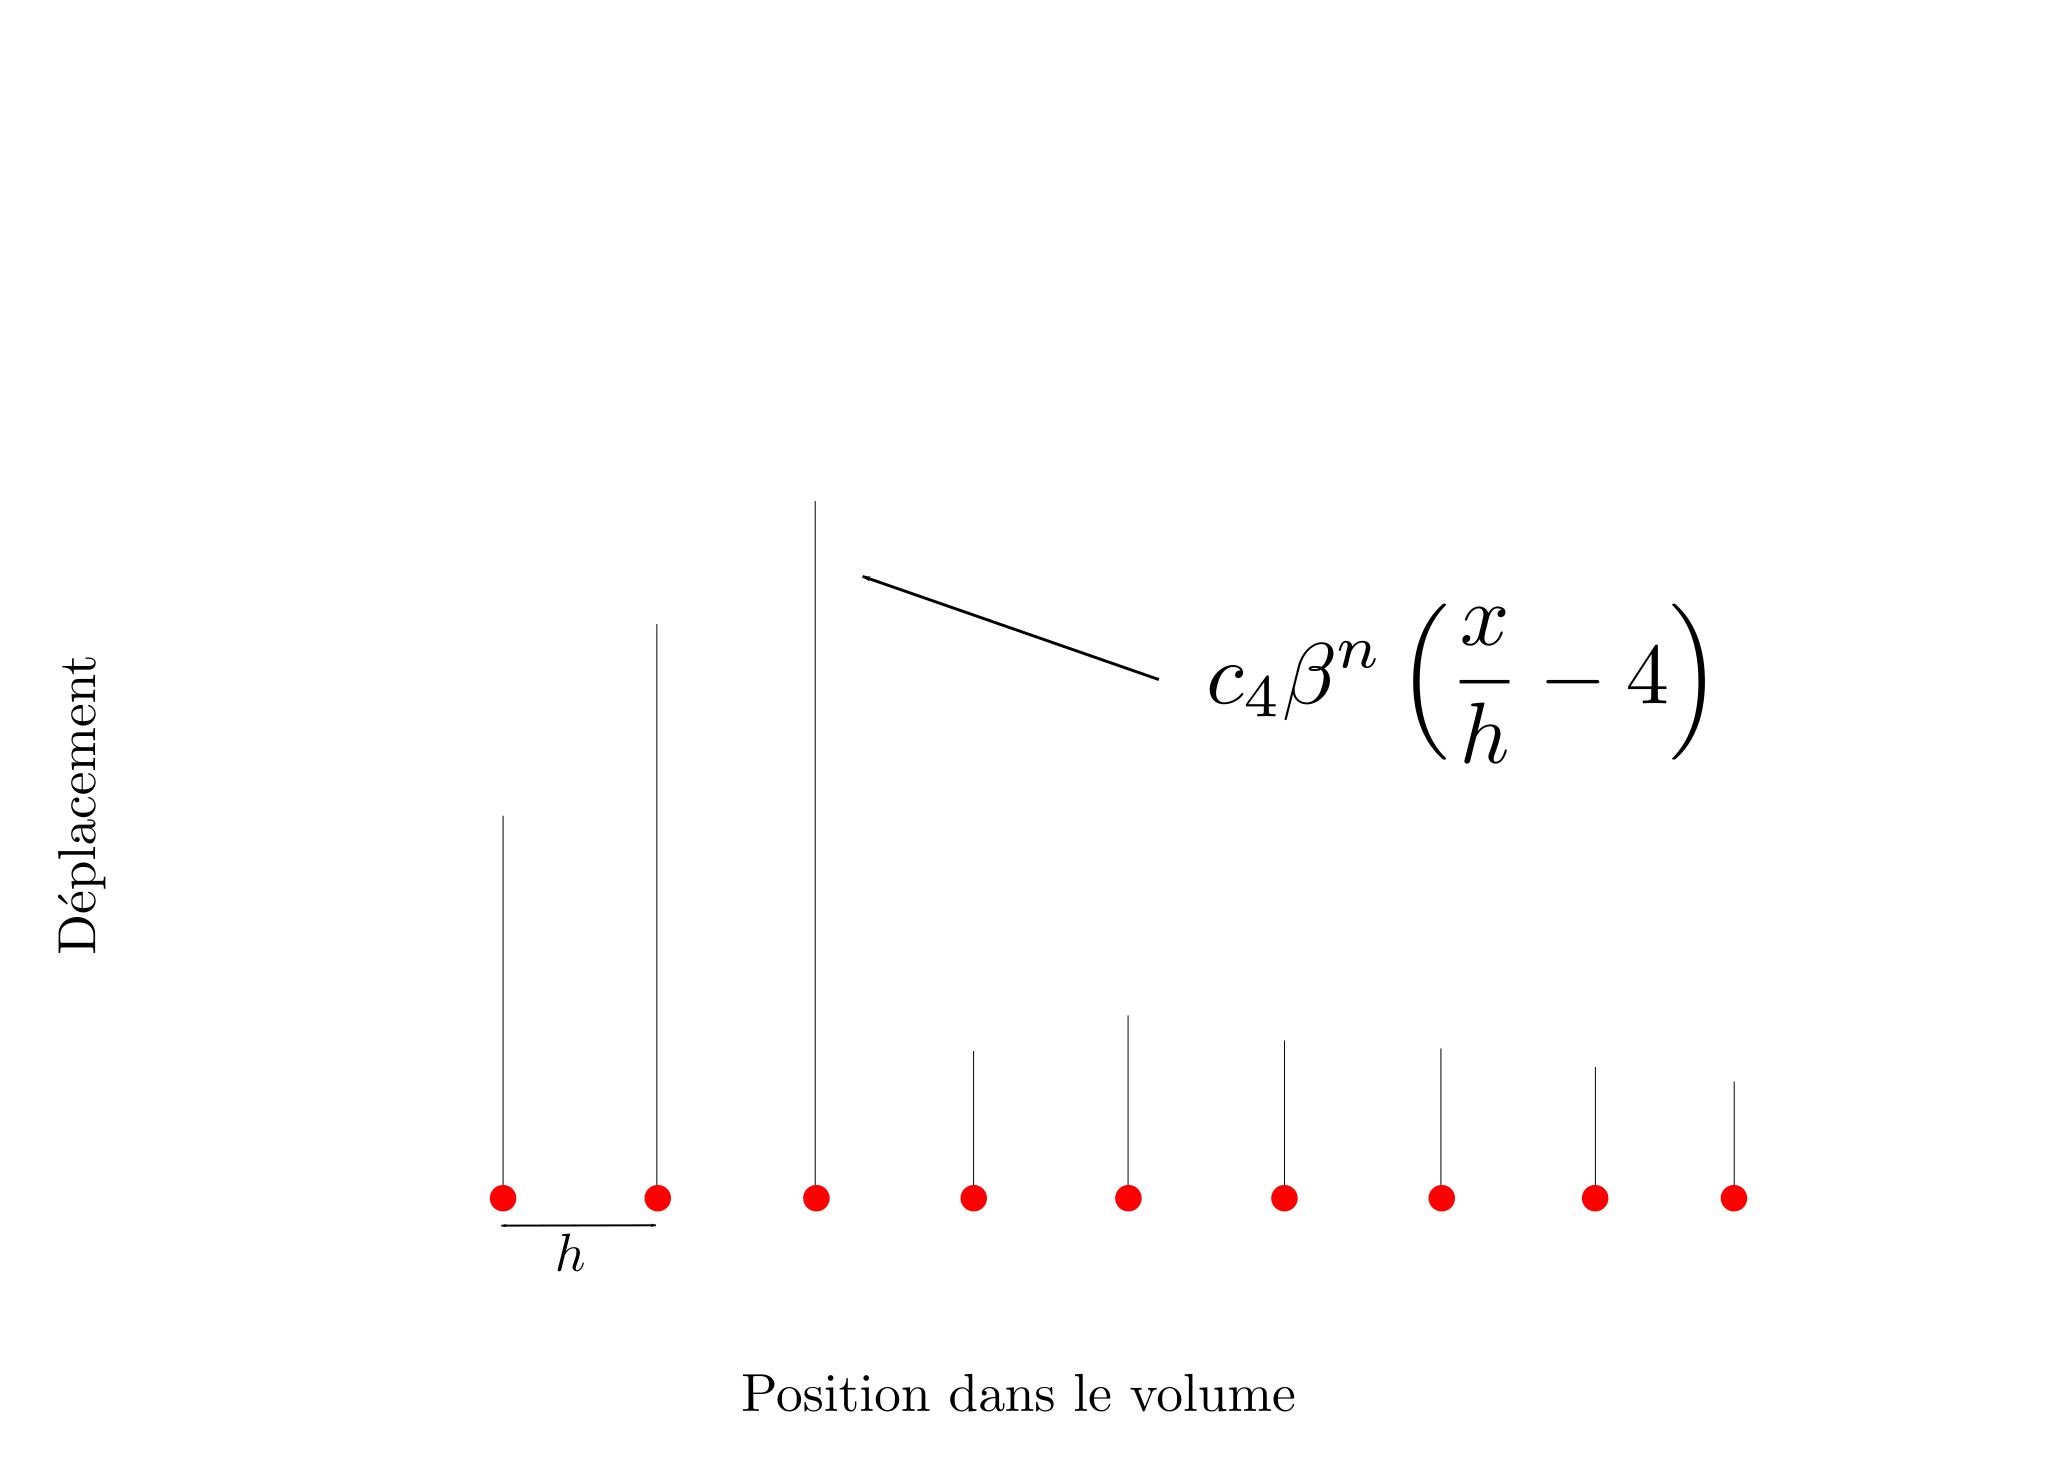
\includegraphics[width=17cm]{images/Bspline}
\caption[Exemple d'interpolation par B-spline]{Exemple d'interpolation par B-spline en 1 dimension : La courbe en trait pointillé épais est représentée par la la somme d'un ensemble de courbes B-spline représentées en traits pointillés fins.}
\label{fig:Bspline}
\end{figure}


\begin{equation}
  g_t(x)=x + \sum\limits_{j\in \mathbb{Z}^N} c_j \beta^n \left( \frac{x}{h}-j \right)
\end{equation}

Où $\beta^n(x)$ est la valeur de la fonction B-spline de degré $n$ au point $x$, et $j$ représente les indices des positions de la grille. $h$ correspond à l'espacement entre les points de la grille. A chaque fonction B-spline de la grille corresponds un coefficient de pondération associé nommé $c_j$ qui représente l'apport de la B-spline correspondante au signal final.

Les coefficients $c_j$ sont obtenus à l'aide d'une optimisation multi-échelle sur 3 niveaux : L'estimation est réalisée sur des images de résolution différente, en se basant sur l'estimation à la résolution $r-1$ pour réaliser celle de l'estimation à la résolution $r$. l'optimisation est réalisée par gradient conjugué selon la méthode de Polak-Ribière~\cite{polak1969note}. Nous avons utilisé l'erreur quadratique moyenne pour comme métrique de recalage. Elle a l'avantage d'être simple, rapide, et de ne pas montrer de discontinuités~\cite{ledesma2005spatio}.


\subsection{Paramètres de l'estimation de mouvement}

Les images utilisées pour l'estimation du mouvement respiratoire ne sont pas reconstruites avec les mêmes paramètres que les images finales. En effet, la quantité de données disponible pour la reconstruction est 8 fois plus faible que celle utilisée pour réaliser les reconstructions d'images. De plus, nous cherchons à optimiser la qualité de l'estimation de mouvement. C'est pour ces raisons que nous avons réalisé une autre étude pour estimer les paramètres de reconstruction optimaux. 

Pour évaluer la performance de chaque jeu de paramètre, nous avons utilisé la vérité terrain pour créer une image d'évaluation pour l'image de référence, ainsi qu'une autre pour l'image ``respirante``. Les images d'évaluation sont créées à partir des fantômes de référence en assignant aux organes étudiés (foie et poumon) une valeur de 1, et une valeur plus importante pour les lésions. Le reste a une valeur de 0. Une illustration est présentée dans la figure~\ref{lab:illustrationRecalage}.a). 

\begin{figure}
\centering
\begin{tabular}{c c}
	\includegraphics[width=5cm]{images/sansCorrection} & \includegraphics[width=5cm]{images/avecCorrection} \\
	a) Cartes non recalées				& b) Cartes recalées
\end{tabular}
\caption[Illustration du recalage obtenu]{Illustration de la pertinence du recalage obtenu à partir de l'estimation de mouvement réalisée sur les images. En vert l'image de référence et en gris l'image du temps correspondant à la différence la plus importante. }
\label{lab:illustrationRecalage}
\end{figure}

L'image d'évaluation correspondant à l'image ''respirante`` est alors recalée sur l'image de référence à l'aide du champ de mouvement élastique calculé précédemment. Nous évaluons ensuite la qualité du recalage en calculant l'écart quadratique moyen entre les deux images d'évaluation~\ref{lab:illustrationRecalage}.b).

\subsubsection{paramètres de l'estimation de mouvement}

Nous avons évalué l'influence de l'échantillonnage spatial des B-spline sur la qualité de l'estimation de mouvement. En effet, si l'espacement entre les nœuds de contrôle est trop important, les mouvements locaux vont interférer entre eux et le résultat ne sera pas valide. De la même manière, en cas d'espacement trop faible, la nature extrêmement bruitée des images va engendrer des micro-mouvements parasites locaux. Pour réduire le bruit, nous appliquons une filtrage gaussien la largeur à mi-hauteur de 6mm à chaque itération.

Nous avons évalué le recalage des reconstructions pour les paramètres suivants :
\begin{description}
 \item[Nombre d'itérations :] Le nombre de sous-ensembles est toujours de 5, mais nous faisons varier le nombre d'itérations de 1 à 7, ce qui représente un nombre d'itérations totales de 5 à 40.
 \item[Précision de la grille :] nous avons évalué les performances de la détection pour 3 taille différentes, allant d'une grille très peu précise de 2 noeuds en x, y et z, à une grille plus précise avec 5 noeuds en x et y, et 10 noeuds en z. Une grille intermédiaire a été évaluée avec 3 noeuds en x et y, ainsi que 5 noeuds en z.
\end{description}

Les résultats sont présentés dans la figure~\ref{fig:perfsFctIterTaille}

\begin{figure}
\centering
\includegraphics[width=12cm]{images/perfsRecalageFctIter-grid_crop}
\caption[Performances de l'estimation de mouvement en fonction de la taille de la grille de recherche]{Performances de l'estimation de mouvement en fonction du nombre d'itérations de la reconstruction selon la taille de la grille utilisée pour l'estimation de mouvement}
\label{fig:perfsFctIterTaille}
\end{figure}

Les résultats nous montrent que les meilleures performances sont obtenues pour la configuration $3 \times 3 \times 5$ avec 3 itérations et 5 subsets.


\subsubsection{Optimisation des paramètres de reconstruction}

Nous avons ensuite souhaité vérifier que la régularisation avait un impact positif sur la qualité du recalage. Nous avons utilisé les paramètres présentés précédemment pour la valider :

\begin{description}
 \item[Nombre d'itérations :] Le nombre de sous-ensembles est toujours de 5, mais nous faisons varier le nombre d'itérations de 1 à 7, ce qui représente un nombre d'itérations totales de 5 à 40.
 \item[Présence ou absence de régularisation pendant la reconstruction :] Une régularisation par filtrage gaussien de largeur à mi-hauteur de 6 mm est appliquée ou non à chaque itération.
\end{description}

Les résultats sont présentés dans la figure~\ref{lab:perfsFctIterReg}. Ils montrent clairement que la régularisation entraîne une amélioration des performances, et que la meilleure estimation de mouvement est réalisée pour une reconstruction de 3 itérations avec 5 sous-ensembles. Nous avons utilisé une grille de 3 noeuds en x et en y, soit un espacement de 17cm, et de 5 noeuds en z, soit un espacement de 7.7 cm.

\begin{figure}
\centering
\includegraphics[width=10cm]{images/perfsRecalageFctIter_crop}
\caption[Performances de l'estimation de mouvement en fonction de la régularisation]{Performances de l'estimation de mouvement en fonction du nombre d'itérations complètes de la reconstruction selon la présence ou l'absence de régularisation pendant la reconstruction. Plus la valeur en ordonnées (mesure de différence) est faible, meilleure et la performance}
\label{lab:perfsFctIterReg}
\end{figure}